% Options for packages loaded elsewhere
\PassOptionsToPackage{unicode}{hyperref}
\PassOptionsToPackage{hyphens}{url}
%
\documentclass[
]{book}
\usepackage{lmodern}
\usepackage{amssymb,amsmath}
\usepackage{ifxetex,ifluatex}
\ifnum 0\ifxetex 1\fi\ifluatex 1\fi=0 % if pdftex
  \usepackage[T1]{fontenc}
  \usepackage[utf8]{inputenc}
  \usepackage{textcomp} % provide euro and other symbols
\else % if luatex or xetex
  \usepackage{unicode-math}
  \defaultfontfeatures{Scale=MatchLowercase}
  \defaultfontfeatures[\rmfamily]{Ligatures=TeX,Scale=1}
\fi
% Use upquote if available, for straight quotes in verbatim environments
\IfFileExists{upquote.sty}{\usepackage{upquote}}{}
\IfFileExists{microtype.sty}{% use microtype if available
  \usepackage[]{microtype}
  \UseMicrotypeSet[protrusion]{basicmath} % disable protrusion for tt fonts
}{}
\makeatletter
\@ifundefined{KOMAClassName}{% if non-KOMA class
  \IfFileExists{parskip.sty}{%
    \usepackage{parskip}
  }{% else
    \setlength{\parindent}{0pt}
    \setlength{\parskip}{6pt plus 2pt minus 1pt}}
}{% if KOMA class
  \KOMAoptions{parskip=half}}
\makeatother
\usepackage{xcolor}
\IfFileExists{xurl.sty}{\usepackage{xurl}}{} % add URL line breaks if available
\IfFileExists{bookmark.sty}{\usepackage{bookmark}}{\usepackage{hyperref}}
\hypersetup{
  pdftitle={Advanced Data Analysis},
  pdfauthor={Mike Nguyen},
  hidelinks,
  pdfcreator={LaTeX via pandoc}}
\urlstyle{same} % disable monospaced font for URLs
\usepackage{color}
\usepackage{fancyvrb}
\newcommand{\VerbBar}{|}
\newcommand{\VERB}{\Verb[commandchars=\\\{\}]}
\DefineVerbatimEnvironment{Highlighting}{Verbatim}{commandchars=\\\{\}}
% Add ',fontsize=\small' for more characters per line
\usepackage{framed}
\definecolor{shadecolor}{RGB}{248,248,248}
\newenvironment{Shaded}{\begin{snugshade}}{\end{snugshade}}
\newcommand{\AlertTok}[1]{\textcolor[rgb]{0.94,0.16,0.16}{#1}}
\newcommand{\AnnotationTok}[1]{\textcolor[rgb]{0.56,0.35,0.01}{\textbf{\textit{#1}}}}
\newcommand{\AttributeTok}[1]{\textcolor[rgb]{0.77,0.63,0.00}{#1}}
\newcommand{\BaseNTok}[1]{\textcolor[rgb]{0.00,0.00,0.81}{#1}}
\newcommand{\BuiltInTok}[1]{#1}
\newcommand{\CharTok}[1]{\textcolor[rgb]{0.31,0.60,0.02}{#1}}
\newcommand{\CommentTok}[1]{\textcolor[rgb]{0.56,0.35,0.01}{\textit{#1}}}
\newcommand{\CommentVarTok}[1]{\textcolor[rgb]{0.56,0.35,0.01}{\textbf{\textit{#1}}}}
\newcommand{\ConstantTok}[1]{\textcolor[rgb]{0.00,0.00,0.00}{#1}}
\newcommand{\ControlFlowTok}[1]{\textcolor[rgb]{0.13,0.29,0.53}{\textbf{#1}}}
\newcommand{\DataTypeTok}[1]{\textcolor[rgb]{0.13,0.29,0.53}{#1}}
\newcommand{\DecValTok}[1]{\textcolor[rgb]{0.00,0.00,0.81}{#1}}
\newcommand{\DocumentationTok}[1]{\textcolor[rgb]{0.56,0.35,0.01}{\textbf{\textit{#1}}}}
\newcommand{\ErrorTok}[1]{\textcolor[rgb]{0.64,0.00,0.00}{\textbf{#1}}}
\newcommand{\ExtensionTok}[1]{#1}
\newcommand{\FloatTok}[1]{\textcolor[rgb]{0.00,0.00,0.81}{#1}}
\newcommand{\FunctionTok}[1]{\textcolor[rgb]{0.00,0.00,0.00}{#1}}
\newcommand{\ImportTok}[1]{#1}
\newcommand{\InformationTok}[1]{\textcolor[rgb]{0.56,0.35,0.01}{\textbf{\textit{#1}}}}
\newcommand{\KeywordTok}[1]{\textcolor[rgb]{0.13,0.29,0.53}{\textbf{#1}}}
\newcommand{\NormalTok}[1]{#1}
\newcommand{\OperatorTok}[1]{\textcolor[rgb]{0.81,0.36,0.00}{\textbf{#1}}}
\newcommand{\OtherTok}[1]{\textcolor[rgb]{0.56,0.35,0.01}{#1}}
\newcommand{\PreprocessorTok}[1]{\textcolor[rgb]{0.56,0.35,0.01}{\textit{#1}}}
\newcommand{\RegionMarkerTok}[1]{#1}
\newcommand{\SpecialCharTok}[1]{\textcolor[rgb]{0.00,0.00,0.00}{#1}}
\newcommand{\SpecialStringTok}[1]{\textcolor[rgb]{0.31,0.60,0.02}{#1}}
\newcommand{\StringTok}[1]{\textcolor[rgb]{0.31,0.60,0.02}{#1}}
\newcommand{\VariableTok}[1]{\textcolor[rgb]{0.00,0.00,0.00}{#1}}
\newcommand{\VerbatimStringTok}[1]{\textcolor[rgb]{0.31,0.60,0.02}{#1}}
\newcommand{\WarningTok}[1]{\textcolor[rgb]{0.56,0.35,0.01}{\textbf{\textit{#1}}}}
\usepackage{longtable,booktabs}
% Correct order of tables after \paragraph or \subparagraph
\usepackage{etoolbox}
\makeatletter
\patchcmd\longtable{\par}{\if@noskipsec\mbox{}\fi\par}{}{}
\makeatother
% Allow footnotes in longtable head/foot
\IfFileExists{footnotehyper.sty}{\usepackage{footnotehyper}}{\usepackage{footnote}}
\makesavenoteenv{longtable}
\usepackage{graphicx,grffile}
\makeatletter
\def\maxwidth{\ifdim\Gin@nat@width>\linewidth\linewidth\else\Gin@nat@width\fi}
\def\maxheight{\ifdim\Gin@nat@height>\textheight\textheight\else\Gin@nat@height\fi}
\makeatother
% Scale images if necessary, so that they will not overflow the page
% margins by default, and it is still possible to overwrite the defaults
% using explicit options in \includegraphics[width, height, ...]{}
\setkeys{Gin}{width=\maxwidth,height=\maxheight,keepaspectratio}
% Set default figure placement to htbp
\makeatletter
\def\fps@figure{htbp}
\makeatother
\setlength{\emergencystretch}{3em} % prevent overfull lines
\providecommand{\tightlist}{%
  \setlength{\itemsep}{0pt}\setlength{\parskip}{0pt}}
\setcounter{secnumdepth}{5}
\usepackage{booktabs}
\usepackage[]{natbib}
\bibliographystyle{apalike}

\title{Advanced Data Analysis}
\author{Mike Nguyen}
\date{2021-01-18}

\begin{document}
\maketitle

{
\setcounter{tocdepth}{1}
\tableofcontents
}
\hypertarget{prerequisites}{%
\chapter{Prerequisites}\label{prerequisites}}

\begin{Shaded}
\begin{Highlighting}[]
\KeywordTok{install.packages}\NormalTok{(}\StringTok{"bookdown"}\NormalTok{)}
\CommentTok{# or the development version}
\CommentTok{# devtools::install_github("rstudio/bookdown")}
\end{Highlighting}
\end{Shaded}

This book's skeleton is based on several courses. Hence, I'd like to credit professors accordingly.

\begin{longtable}[]{@{}cc@{}}
\toprule
Course & Professor\tabularnewline
\midrule
\endhead
Analyzing Unstructured Data & Kunpeng Zhang\tabularnewline
Deep Learning & Yann LeCun\tabularnewline
\bottomrule
\end{longtable}

Compare to the last \href{https://bookdown.org/mike/data_analysis/}{book}, this book should differ as follows:

\hypertarget{part-machine-learning}{%
\part{MACHINE LEARNING}\label{part-machine-learning}}

\hypertarget{intro}{%
\chapter{Introduction}\label{intro}}

3 types of data

\begin{itemize}
\tightlist
\item
  Structured Data (tables form)\\
\item
  Semi-structured Data (e.g., XML, JSON, HTML)\\
\item
  Unstructured Data

  \begin{itemize}
  \tightlist
  \item
    Texts\\
  \item
    Images: Videos, photos,\\
  \item
    Networks: Social Networks
  \end{itemize}
\end{itemize}

\hypertarget{machine-learning}{%
\chapter{Machine Learning}\label{machine-learning}}

This section based on notes in ``Analyzing Unstructured Data'' course taught by professor Kunpeng Zhang.

\begin{itemize}
\tightlist
\item
  ML is concerned with the the development, the analysis, and the application of algorithm that allow computers to learn\\
\item
  Learning:

  \begin{itemize}
  \tightlist
  \item
    A computer learns if it improves its performance at some tasks with experience (i.e., data)\\
  \item
    Extracting a model of system from the sole observation (or the simulation)\\
  \item
    A model = some relationships between the variables used to describe the system.\\
  \end{itemize}
\item
  Goals:

  \begin{itemize}
  \tightlist
  \item
    Make prediction\\
  \item
    Understand the underlying mechanisms.\\
  \end{itemize}
\item
  Learning if useful when:

  \begin{itemize}
  \tightlist
  \item
    Human expertise does not exist (navigating on Mars)\\
  \item
    Humans are unable to explain their expertise (speech recognition)\\
  \item
    Solution changes in time (routing on a computer network)\\
    Solution needs to be adapted to particular cases (user biometrics)\\
  \end{itemize}
\item
  Applications in different domains:

  \begin{itemize}
  \tightlist
  \item
    Retail: Market basket analysis, customer relationship management (CRM)\\
  \item
    Finance: Credit scoring, fraud detection.\\
  \item
    Manufacturing: Optimization, troubleshooting\\
  \item
    Medicine: medical diagnosis\\
  \item
    Telecommunications: Quality of service optimization, routing\\
  \item
    Bioinformatics: Motifs, alignment WEb mining, search engines.\\
  \end{itemize}
\item
  Steps

  \begin{itemize}
  \tightlist
  \item
    Data generation: data types, sample size\\
  \item
    Preprocessing: normalization, missing values, feature selection/extraction\\
  \item
    Machine Learning: Hypothesis, choice of learning paradigm/algorithm.\\
  \item
    Hypothesis validation: cross-validation, model deployment.\\
  \end{itemize}
\item
  Types of machine learning:

  \begin{itemize}
  \tightlist
  \item
    Supervised: manually label variables\\
  \item
    Unsupervised:\\
  \end{itemize}
\item
  Training and testing

  \begin{itemize}
  \tightlist
  \item
    Training is the process of making the machine learn\\
  \item
    No free lunch:

    \begin{itemize}
    \tightlist
    \item
      Training set and testing set come from the same distribution\\
    \item
      Need to make some assumptions.\\
    \end{itemize}
  \end{itemize}
\item
  Factors affecting the performance:

  \begin{itemize}
  \tightlist
  \item
    Types of training provided\\
  \item
    The form and extend of prior knowledge\\
  \item
    Type of feedback provided\\
  \item
    The learning algorithms used\\
  \end{itemize}
\item
  Two factors:

  \begin{itemize}
  \tightlist
  \item
    Modeling\\
  \item
    optimization\\
  \end{itemize}
\item
  Algorithms:

  \begin{itemize}
  \tightlist
  \item
    ML depends on algorithms.\\
  \item
    The algorithms control the search to find and build the knowledge structures\\
  \item
    The learning algorithms should extract useful information from training examples.\\
  \end{itemize}
\item
  Types of learning (algorithms):

  \begin{itemize}
  \tightlist
  \item
    Supervised learning (\(\{ X_n \in R^d, y_n \in R\}^N_{n=1}\))

    \begin{itemize}
    \tightlist
    \item
      Prediction\\
    \item
      Classification (discrete labels), regression (real values)\\
    \end{itemize}
  \item
    Unsupervised learning (\(\{ X_n \in R^d\}^N_{n=1}\))

    \begin{itemize}
    \tightlist
    \item
      Clustering\\
    \item
      Probability distribution estimation\\
    \item
      Finding association (in features)\\
    \item
      Dimension reduction\\
    \end{itemize}
  \item
    Semi-supervised learning\\
  \item
    Reinforcement learning

    \begin{itemize}
    \tightlist
    \item
      Decision making (robot, chess machine)
    \end{itemize}
  \end{itemize}
\end{itemize}

\hypertarget{supervised-learning}{%
\section{Supervised Learning}\label{supervised-learning}}

From the data, find a function f of the inputs that best approximates the outputs.

\[
\hat{Y} = f(X_1,..,X_n)
\]

\begin{itemize}
\tightlist
\item
  Predictive: Make predictions for a new object described by its attributes\\
\item
  Informative: help understand the relationship between inputs and outputs
\end{itemize}

Divide data into

\begin{itemize}
\tightlist
\item
  Training set: train model\\
\item
  validation set: tune hyper parameters\\
\item
  Test set: evaluation of the model for generalization error.
\end{itemize}

Learning algorithm

\begin{itemize}
\tightlist
\item
  defined by

  \begin{itemize}
  \tightlist
  \item
    a family of candidate models (= \textbf{hypothesis space H})\\
  \item
    a quality measure for a model\\
  \item
    an optimization strategy\\
  \end{itemize}
\item
  takes as input a leaning sample and outputs a function h in H of maximum quality
\end{itemize}

Model selection

\begin{itemize}
\tightlist
\item
  Why not choose the model that minimizes the error rate on the learning sample? (\textbf{re-substitution error})\\
\item
  How well are you going to predict future data drawn from the same distribution? (\textbf{generalization error})
\item
  Evaluation on test set

  \begin{enumerate}
  \def\labelenumi{\arabic{enumi}.}
  \tightlist
  \item
    Randomly choose a percentage (e.g., 30\%) of the data to be in a test set\\
  \item
    The remainder is training set\\
  \item
    Learn the model from the training set\\
  \item
    Estimate its future performance on the test set.\\
  \end{enumerate}
\item
  Problems:

  \begin{itemize}
  \tightlist
  \item
    overfits: occurs when the learning algorithm starts fitting noise.\\
  \item
    unfits\\
  \end{itemize}
\item
  Evaluation on test set:

  \begin{itemize}
  \tightlist
  \item
    Good:

    \begin{itemize}
    \tightlist
    \item
      Very simple\\
    \item
      Computationally efficient\\
    \end{itemize}
  \item
    Bad:

    \begin{itemize}
    \tightlist
    \item
      Waste data\\
    \item
      very unstable when database is small\\
    \end{itemize}
  \end{itemize}
\item
  Another evaluation: \textbf{Leave-one-out cross validation}

  \begin{itemize}
  \tightlist
  \item
    For k = 1 to N

    \begin{itemize}
    \tightlist
    \item
      remove the k-th object from the learning sample\\
    \item
      learn the model on the remaining objects\\
    \item
      apply the model to get a prediction for the k-th object\\
    \end{itemize}
  \item
    report the proportion of mis-classified objects\\
  \end{itemize}
\item
  Good:

  \begin{itemize}
  \tightlist
  \item
    Do not waste the data (you get an estimate of the best method to apply to N-1 data)\\
  \end{itemize}
\item
  Bad:

  \begin{itemize}
  \tightlist
  \item
    Computationally intensive (train N models)\\
  \item
    high variance.\\
  \end{itemize}
\item
  Another evaluation: \textbf{K-fold cross validation}:

  \begin{itemize}
  \tightlist
  \item
    Break up data into k folds\\
  \item
    For each fold

    \begin{itemize}
    \tightlist
    \item
      Choose the fold as a temporary test set\\
    \item
      Train on k-1 folds, compute performance on the test fold.\\
    \end{itemize}
  \item
    Report average performance of the 10 runs.\\
  \item
    randomly partition the dataset into k subsets (e.g., 10)\\
  \item
    For each subset:

    \begin{itemize}
    \tightlist
    \item
      learn the model on the objects that are not in the subset\\
    \item
      compute the error rate on the points in the subset. Report the mean error rate over the k subsets.\\
    \end{itemize}
  \item
    When k = the number of objects -\textgreater{} leave-one-out-cross validation.
  \end{itemize}
\end{itemize}

Rule-of-thumb for evaluation

\begin{itemize}
\tightlist
\item
  Lots of data (\textgreater1000) test set validation\\
\item
  small data (100-1000): 10-fold CV\\
\item
  very small data (\textless100) leave one out CV.
\end{itemize}

\begin{center}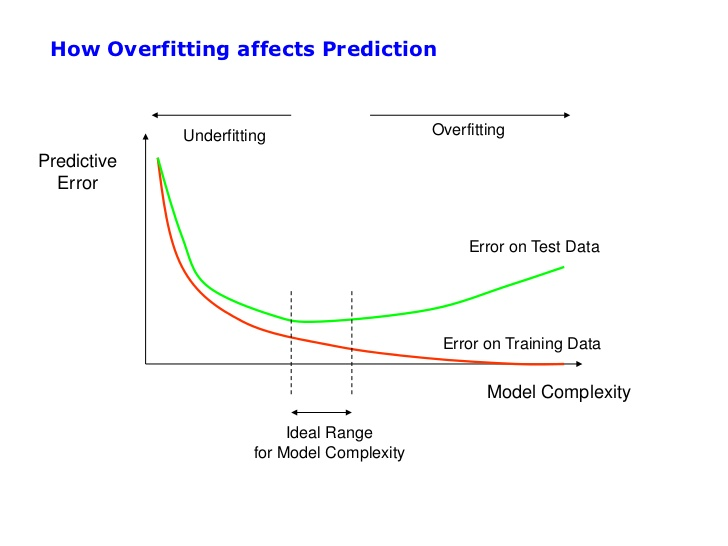
\includegraphics[width=10.11in]{images/Overfitting affect prediction} \end{center}

Use the testing set to estimate the performance of the final model

Performance measures

\begin{itemize}
\tightlist
\item
  The error rate is no the only way to assess a predictive model.\\
\item
  In binary classification, results can be summarized in a contingency table (i.e., confusion matrix)
\end{itemize}

\begin{center}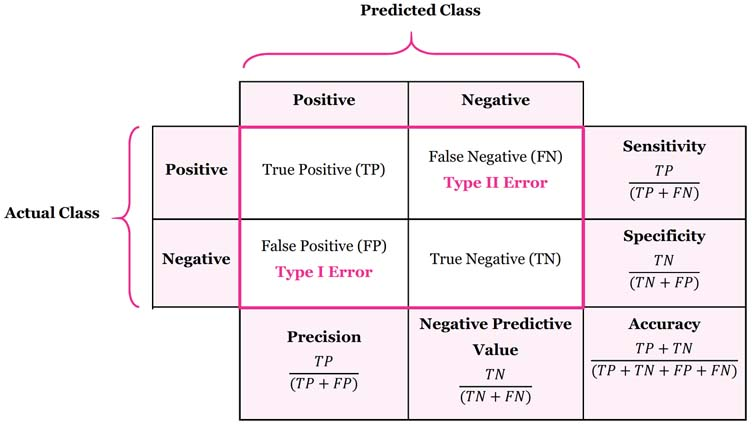
\includegraphics[width=10.47in]{images/confusionMatrxiUpdated} \end{center}

Various criteria

\[
\text{Error rate} = \frac{FP + FN}{N + P} \\
\text{Accuracy} = \frac{TP + TN}{N + P} = 1 - \text{Error rate} \\
\text{Sensitivity or recall} = \frac{TP}{P} \\
\text{Specificity} = \frac{TN}{TN + FP} \\
\text{Precision} = \frac{TP}{TP + FP} \\
\]

\textbf{ROC and precision/recall curves}

\begin{itemize}
\tightlist
\item
  Each point corresponds to a particular choice of the decision threshold.
\end{itemize}

Also known as robustness check

You want large area under the curve

Compassion of learning models

\begin{itemize}
\tightlist
\item
  Three main criteria:

  \begin{itemize}
  \tightlist
  \item
    Accuracy: Measures by the generalization error (estimated by CV)\\
  \item
    Efficiency: Computing times and scalabiility for learning and testing\\
  \item
    Interpretability: Comprehension brought by the model about the input-output relationship.\\
  \end{itemize}
\item
  Depends on the application, you have to make trade-off.
\end{itemize}

Learning Techniques

\begin{itemize}
\tightlist
\item
  Supervised learning categories and techniques

  \begin{itemize}
  \tightlist
  \item
    Linear classifier (numerical functions):

    \begin{itemize}
    \tightlist
    \item
      Perceptron\\
    \item
      Logistic regression\\
    \item
      Support vector machine (SVM): linear to nonlinear: feature transofrm and kernel function\\
    \item
      Ada-line\\
    \item
      Multi-layer perceptron (MLP)
    \end{itemize}
  \item
    Parametric (Probabilistic functions)

    \begin{itemize}
    \tightlist
    \item
      Naive Bayes, Gaussian discriminant analysis (GDA), Hidden Markov models (HMM), probabilistic graphical models\\
    \end{itemize}
  \item
    Non-parametric (Instance-based functions)

    \begin{itemize}
    \tightlist
    \item
      K-nearest neighbors, Kernel regression, Kernel density estimation, local regression.\\
    \end{itemize}
  \item
    Non-metric (symbolic functions)

    \begin{itemize}
    \tightlist
    \item
      Classification and regression tree (CART), decision tree\\
    \end{itemize}
  \item
    Aggregation

    \begin{itemize}
    \tightlist
    \item
      Bagging (bootstrap + aggregation), Adaboost, Random forest.\\
    \end{itemize}
  \end{itemize}
\item
  Unsupervised learning categories and techniques:

  \begin{itemize}
  \tightlist
  \item
    Clustering

    \begin{itemize}
    \tightlist
    \item
      K-means clustering\\
    \item
      Spectral clustering\\
    \end{itemize}
  \item
    Density Estimation

    \begin{itemize}
    \tightlist
    \item
      Gaussian mixture model (GMM)\\
    \item
      Graphical models\\
    \end{itemize}
  \item
    Dimensionality reduction

    \begin{itemize}
    \tightlist
    \item
      Principal component analysis (PCA)\\
    \item
      Factor analysis\\
    \end{itemize}
  \end{itemize}
\item
  Semi-supervised learning

  \begin{itemize}
  \tightlist
  \item
    goal: exploit both labeled and unlabeled data to build better models than using each one alone\\
  \item
    Self-training:

    \begin{itemize}
    \tightlist
    \item
      Iteratively label some unlabeled examples with a model learned from the previously labeled examples\\
    \item
      Active learning.\\
    \end{itemize}
  \end{itemize}
\item
  Reinforcement learning

  \begin{itemize}
  \tightlist
  \item
    Learning from interactions\\
  \item
    Goal: learn to choose sequence of actions (=policy) that maximizes \(r_0 + \gamma r_1 + \gamma^2r_2 + ...\) where \(0 \le \gamma <1\)
  \end{itemize}
\end{itemize}

\hypertarget{decision-tree}{%
\subsection{Decision Tree}\label{decision-tree}}

\begin{itemize}
\tightlist
\item
  Is a tree-structured plan of a set of attributes to test to predict the output.\\
\item
  Give one attribute, try to predict the value of new people's attribute by means of some other available attribute\\
\item
  Input attributes:

  \begin{itemize}
  \tightlist
  \item
    \textbf{d} features/ attributes \(x^{(1)},x^{(2)},...,x^{(d)}\)\\
  \item
    Each \(x^{(j)}\) has domain \(O_j\)

    \begin{itemize}
    \tightlist
    \item
      Categorical \(O_j=(read,blue)\)\\
    \item
      Numerical: \(H_j = (0,10)\)\\
    \end{itemize}
  \item
    Y is output variable with domain \(O_Y\):

    \begin{itemize}
    \tightlist
    \item
      Categorical: Classification\\
    \item
      Numerical: regression\\
    \end{itemize}
  \end{itemize}
\item
  Data D:

  \begin{itemize}
  \tightlist
  \item
    n examples \((x_i, y_i)\) where

    \begin{itemize}
    \tightlist
    \item
      \(x_i\) is a d-dim feature vector\\
    \item
      \(y_i\in O_Y\)\\
    \end{itemize}
  \end{itemize}
\item
  Decision trees:

  \begin{itemize}
  \tightlist
  \item
    Split the data at each internal node
  \item
    Each leaf node makes a prediction
  \end{itemize}
\end{itemize}

How to construct a tree

\begin{itemize}
\tightlist
\item
  \protect\hyperlink{find-best-split}{Find best split}\\
\item
  \protect\hyperlink{stopping-criteria}{Stopping Criteria}\\
\item
  \protect\hyperlink{find-prediction}{Find Prediction}
\end{itemize}

\hypertarget{find-best-split}{%
\subsubsection{Find best split}\label{find-best-split}}

Pick an attribute and value that optimizes some criterion\\
+ Regression: Purity
+ Classification: Information Gain: Measures how much a given attribute X tells us about the class Y.

Information Gain? Entropy

The entropy of X: \(H(X) = -\sum_{j=1}^{m} p_j log p_j\)

\begin{itemize}
\tightlist
\item
  ``High entropy'': X is from a uniform distribution

  \begin{itemize}
  \tightlist
  \item
    A histogram of the frequency distribution of values of X is flat\\
  \end{itemize}
\item
  ``Low Entropy'': X is from varied distribution

  \begin{itemize}
  \tightlist
  \item
    A histogram of the frequency distribution of values of X would have many lows and one or two highs.\\
  \end{itemize}
\item
  Def: Information Gain:

  \begin{itemize}
  \tightlist
  \item
    \(IG(Y|X) = H(Y) - H(Y|X)\) I must transmit Y. How many bits on average would it save me if both ends of the line knew X?
  \end{itemize}
\end{itemize}

\hypertarget{stopping-criteria}{%
\subsubsection{Stopping Criteria}\label{stopping-criteria}}

\begin{itemize}
\tightlist
\item
  When the leaf is ``pure'': the target variable does not vary too much: Var(Y) \textless{} threshold.\\
\item
  When number of examples in the leaf is too small.\\
\item
  Could also use information as as a stopping criteria.
\end{itemize}

\hypertarget{find-prediction}{%
\subsubsection{Find Prediction}\label{find-prediction}}

\begin{itemize}
\tightlist
\item
  Regression: Predict average y of the examples\\
\item
  Classification: Predict most common y of the examples the leaf.
\end{itemize}

\hypertarget{random-forest}{%
\subsection{Random Forest}\label{random-forest}}

Ensemble methods

\begin{itemize}
\tightlist
\item
  A single decision tree does not perform well.\\
\item
  But, it is super fast.\\
\item
  What if we learn multiple trees?
\end{itemize}

Bagging

\begin{itemize}
\tightlist
\item
  If we split the data in random different ways, decision trees give different results, high variance.\\
\item
  Bagging: Bootstrap aggregating is a method that result in low variance.\\
\item
  If we had multiple realizations of the data (or multiple samples) we could calculate the prediction multiple times and take the average of the fact that averaging multiple onerous estimations produce less uncertain results\\
\item
  say for each sample b, we calculate \(f^b(x)\), then \(\hat{f}_{avg} (x) = \frac{1}{B} \sum_{b=1}^{B} \hat{f}^b (x)\)
\item
  Bootstrap: Construct B (hundreds) of trees. Learn a classifier for each bootstrap sample and average them. Very effective.\\
\item
  Reduces overfitting (variance)\\
\item
  Could use one classifier, or multiple classifiers.
\item
  easy to parallelize\\
\item
  Variable Importance Measures

  \begin{itemize}
  \tightlist
  \item
    Bagging results in improved accuracy over prediction using a single tree\\
  \item
    Unfortunately, difficult to interpret the resulting model. Bagging improves prediction accuracy at the expense of interpretability.\\
  \end{itemize}
\item
  Issues:

  \begin{itemize}
  \tightlist
  \item
    Each tree is identically distributed (i.d)

    \begin{itemize}
    \tightlist
    \item
      The expectation of the average of B such trees\\
    \item
      The bias of bagged trees is the same as that of individual trees
    \end{itemize}
  \item
    An average of B i.i.d random variables, each with variance \(\sigma^2\), has variance \(\sigma^2/B\). If i.d. (identical but not independent) and pair correlation \(\rho\) is present, then the variance is : \(\rho \sigma^2 + \frac{1-\rho}{B} \sigma^2\) . As B increases, the second term disappears but the first term remains.\\
  \end{itemize}
\item
  Suppose that there is one very strong predictor in the data set, along with a number of other moderately strong predictors. Then all bagged trees will select the strong predictor at the top tree and therefore all trees will look similar.

  \begin{itemize}
  \tightlist
  \item
    We can penalize the splitting with a penalty term that depends on the number of times a predictor is selected at a given length.\\
  \item
    restrict how many items a predictor can be used.\\
  \item
    allow a certain number of predictors.\\
  \end{itemize}
\item
  Since we want i.i.d so that the bias to be the same and variance to be less.

  \begin{itemize}
  \tightlist
  \item
    in bagging, we build a number of decision trees on bootstrapped training samples each time a split in a tree is considered, a random sample of m predictors is chosen as split candidates from the full set of p predictors (if m = p, then this is bagging).
  \end{itemize}
\end{itemize}

\href{http://www.stat.berkeley.edu/~breiman/RandomForests/}{Random Forest software}

Random Forests Algorithm

For b = 1 to B:

\begin{enumerate}
\def\labelenumi{\alph{enumi}.}
\tightlist
\item
  draw a bootstrap sample Z * of size N from the training data.\\
\item
  Grow a random-forest tree to the bootstrapped data, by recursively repeating the following steps for each terminal node of the tree, until the minimum node size \(n_{min}\) is reached.

  \begin{itemize}
  \tightlist
  \item
    Select m variables at random from the p variables.\\
  \item
    Pick the best variable/split-point among the m.\\
  \item
    Split the node into two daughter nodes.
  \end{itemize}
\end{enumerate}

Output the ensemble trees.

\begin{longtable}[]{@{}lll@{}}
\toprule
\begin{minipage}[b]{0.30\columnwidth}\raggedright
\strut
\end{minipage} & \begin{minipage}[b]{0.30\columnwidth}\raggedright
Regression\strut
\end{minipage} & \begin{minipage}[b]{0.30\columnwidth}\raggedright
Classification\strut
\end{minipage}\tabularnewline
\midrule
\endhead
\begin{minipage}[t]{0.30\columnwidth}\raggedright
To make a prediction at a new point x\strut
\end{minipage} & \begin{minipage}[t]{0.30\columnwidth}\raggedright
average the results\strut
\end{minipage} & \begin{minipage}[t]{0.30\columnwidth}\raggedright
majority vote\strut
\end{minipage}\tabularnewline
\begin{minipage}[t]{0.30\columnwidth}\raggedright
Tuning\strut
\end{minipage} & \begin{minipage}[t]{0.30\columnwidth}\raggedright
The default value for m is \(p/3\) and the minimum node size is 5\strut
\end{minipage} & \begin{minipage}[t]{0.30\columnwidth}\raggedright
The default value for m is \(\sqrt{p}\) and the minimum node size is one\strut
\end{minipage}\tabularnewline
\bottomrule
\end{longtable}

Another issue:

When the number of variables is large, but the fraction of relevant variables is small, random forests are likely to perform poorly when m is small. Because: At each split the chance can be small that the relevant variables will be selected.

Example: with 3 relevant and 100 not so relevant variables the probability of any of the relevant variables being selected at any split is approx 0.25.

random forests ``cannot overfit'' the data because the number of trees (B) does not mean increase in the flexibility of the model.

Always include Random Forest (ensembles) and XGBoost (like bagging)

Alternative

\begin{itemize}
\tightlist
\item
  Support vector machine (SVM) dont usually use this because of computational reasons and because it is only 1 model.
\end{itemize}

\hypertarget{unsupervised-learning}{%
\section{Unsupervised Learning}\label{unsupervised-learning}}

Unsupervised learning tries to find regularities in the data without guidance about inputs and outputs

Unsupervised learning categories and techniques:

\begin{itemize}
\tightlist
\item
  Clustering

  \begin{itemize}
  \tightlist
  \item
    K-means Clustering\\
  \item
    Spectral Clustering\\
  \end{itemize}
\item
  Density Estimation

  \begin{itemize}
  \tightlist
  \item
    Gaussian mixture model (GMM)\\
  \item
    Graphical models\\
  \end{itemize}
\item
  Dimensionality reduction

  \begin{itemize}
  \tightlist
  \item
    Principal component analysis (PCA)\\
  \item
    factor Analysis
  \end{itemize}
\end{itemize}

\hypertarget{clustering}{%
\subsection{Clustering}\label{clustering}}

Clustering is used to find similar groups in data (i.e., clusters)

No class value denoting an a priori grouping (hence, \protect\hyperlink{unsupervised-learning}{Unsupervised Learning})

Clustering algorithm

\begin{itemize}
\tightlist
\item
  Partitional clustering\\
\item
  Hierarchical clustering
\end{itemize}

A distance (similarity, or dissimilarity) function

Clustering quality

\begin{itemize}
\tightlist
\item
  Inter-clusters distance -\textgreater{} maximized\\
\item
  Intra-clusters distance -\textgreater{} minimized
\end{itemize}

which can be use to judge good clustering

\begin{itemize}
\tightlist
\item
  Internal criterion: A good clustering will produce high quality clusters in which:

  \begin{itemize}
  \tightlist
  \item
    The intra-class (intra-cluster) similarity is high\\
  \item
    The inter-class similarity is low.\\
  \item
    The measured quality of a clustering depends on both the document representation and the similarity measure used.\\
  \end{itemize}
\item
  External criteria:

  \begin{itemize}
  \tightlist
  \item
    Quality measured by its ability to discover some or all of the hidden patterns or latent classes in gold standard data.\\
  \item
    Assesses a clustering with respect to \textbf{ground truth}\\
  \item
    Assume documents with C gold standard classes, while our clustering algorithm produce cluster \(w_1,w_2,...,w_k\) with \(n_1,...,n_k\) members.\\
  \item
    Simple measure: \textbf{purity}, the ratio between the dominant class in the cluster \(\pi_i\) and the size of cluster \(w_i\)\\
    \[
    Purity(w_i) = \frac{1}{n_i}max_j (n_{ij})  j \in C
    \]
  \item
    others are entropy of classes in clusters (or mutual inforamtion between classes and clusters).
  \end{itemize}
\end{itemize}

The quality of a clustering result depends on

\begin{itemize}
\tightlist
\item
  The algorithm\\
\item
  the distance function\\
\item
  the application
\end{itemize}

\hypertarget{similarity-measures}{%
\subsubsection{Similarity Measures}\label{similarity-measures}}

It's your choice of how to define similarity

(Dis)similarity measure

\begin{itemize}
\tightlist
\item
  Equivalently, we can use dissimilarity measures\\
\item
  Jagota defines a dissimilarity measure as a function f(x,y) such that f(x,y) \textgreater{} f(w,z) if and only if x is less similar to y than w is to z.\\
  Also known as \textbf{pair-wise} measure
\end{itemize}

Distance functions

Different distance functions for

\begin{itemize}
\tightlist
\item
  Different types of data

  \begin{itemize}
  \tightlist
  \item
    Numeric data\\
  \item
    Nominal data\\
  \end{itemize}
\item
  Different applications
\end{itemize}

Numeric data

\begin{itemize}
\tightlist
\item
  \(dist(x_i, x_j)\),where

  \begin{itemize}
  \tightlist
  \item
    \(dist(x_j, x_j) = ((x_{i1} - x_{j1})^h + (x_{i2} - x_{j2})^h + ... + (x_{ir} - x_{jr})^h)^{\frac{1}{h}}\)
  \item
    \(x_i\) and \(x_j\) are data points (vectors)\\
  \end{itemize}
\item
  Euclidean distance

  \begin{itemize}
  \tightlist
  \item
    If h = 2, it is the Euclidean distance: \(dist(x_j, x_j) = ((x_{i1} - x_{j1})^2 + (x_{i2} - x_{j2})^2 + ... + (x_{ir} - x_{jr})^2)^{\frac{1}{2}}\)
  \item
    Weighted Euclidean distance: \(dist(x_j, x_j) = (w_1(x_{i1} - x_{j1})^2 + w_2(x_{i2} - x_{j2})^2 + ... + w_r(x_{ir} - x_{jr})^2)^{\frac{1}{2}}\)
  \item
    Squared Eulidean distance: to place progressively greater weight on data points that are further apart: \(dist(x_j, x_j) = (x_{i1} - x_{j1})^2 + (x_{i2} - x_{j2})^2 + ... + (x_{ir} - x_{jr})^2\)
  \end{itemize}
\item
  Manhattan distance

  \begin{itemize}
  \tightlist
  \item
    If h = 1, it is the Manhattan distance: \(dist(x_j, x_j) = |x_{i1} - x_{j1}| + |x_{i2} - x_{j2}| + ... + |x_{ir} - x_{jr}|\)
  \end{itemize}
\item
  Minkowski distance (h is positive integer)

  \begin{itemize}
  \tightlist
  \item
    \(dist(x_j, x_j) = ((x_{i1} - x_{j1})^h + (x_{i2} - x_{j2})^h + ... + (x_{ir} - x_{jr})^h)^{\frac{1}{h}}\)
  \item
    1st dimension, 2nd dimension, etc.\\
  \end{itemize}
\item
  Chebychev distance: define 2 data points as ``different'' if they are different on any one of the attributes

  \begin{itemize}
  \tightlist
  \item
    \(dist(x_j, x_j) = max(|x_{i1} - x_{j1}| + |x_{i2} - x_{j2}| + ... + |x_{ir} - x_{jr}|)\)
  \end{itemize}
\end{itemize}

Binary and nominal Attributes

\begin{itemize}
\tightlist
\item
  Binary attribute: has 2 values or states but no ordering relationship (e.g., gender)\\
\item
  We use a confusion matrix to introduce the distance function/measures\\
\item
  Let the i-th and j-th data points be \(X_i\) and \(x_j\) (vectors)
\end{itemize}

Confusion matrix

\begin{longtable}[]{@{}lllll@{}}
\toprule
& & Data point j & &\tabularnewline
\midrule
\endhead
& & 1 & 0 &\tabularnewline
Data point i & 1 & a & b & a + b\tabularnewline
& 0 & c & d & c + d\tabularnewline
& & a + c & b + d & a + b + c + d\tabularnewline
\bottomrule
\end{longtable}

\begin{itemize}
\tightlist
\item
  a: the number of attributes with the value of 1 for both data points\\
\item
  b: The number of attributes with which \(x_{if} = 1\) and \(x_{jf}=0\) where \(x_{if}\) is the value of \(f\) attribute of the data point \(x_i\)\\
\item
  c: the number of attributes of which \(x_{if}=0\) and \(x_{jf} =1\)\\
\item
  d: the number of attributes with the value of 0 for both data points.
\end{itemize}

Symmetric binary attributes

\begin{itemize}
\tightlist
\item
  A binary attribute is symmetric if both of its states (0 and 1) have equal importance, and carry the same weights, e.g., Gender.\\
\item
  distance function: \textbf{Simple Matching Coefficient}, proportion of mismatches of their values\\
  \[
  dist(x_i,x_j) = \frac{b+c}{a+b+c+d}
  \]
\end{itemize}

Asymmetric binary attributes

\begin{itemize}
\tightlist
\item
  if one of the states is more important or more valuable than the other

  \begin{itemize}
  \tightlist
  \item
    By convention, state 1 represents the more important state.\\
  \item
    Jaccard coefficient is popular measure\\
    \[
    dist(x_i,x_j) = \frac{b + c}{a + b +c}
    \]
  \item
    We can have some variations, adding weights
  \end{itemize}
\end{itemize}

Nominal attributes: with more than 2 states or values.\\
* the common used distance measure is also based on the simple matching method.\\
* Given two data points \(x_i\), \(x_j\) let the number of attributes be r, and the number of values that match in \(x_i\) and \(x_j\) be q. \(dist(x_i,x_j) = \frac{r-q}{r}\)

Data standardization

\begin{itemize}
\tightlist
\item
  In the Euclidean space, standardization of attributes is recommended so that all attributes can have equal impact on the computation of distances.\\
\item
  standardize attributes: to force the attributes to have a common value range.\\
\item
  Real data have different types:

  \begin{itemize}
  \tightlist
  \item
    Interval-scaled
  \item
    symmetric binary\\
  \item
    asymmetric binary\\
  \item
    ratio-scaled\\
  \item
    ordinal\\
  \item
    nominal\\
  \end{itemize}
\item
  Convert to a single type:

  \begin{itemize}
  \tightlist
  \item
    To deal with mixed attributes:

    \begin{itemize}
    \tightlist
    \item
      Decide the dominant attribute type\\
    \item
      Convert the other types to this type
    \end{itemize}
  \end{itemize}
\end{itemize}

\hypertarget{k-mean-algorithm}{%
\subsubsection{K-mean Algorithm}\label{k-mean-algorithm}}

K-means is a partitional clustering algorithm.

Let the set of data points (or instances) D to be \((x_1,...,x_n)\), where \(x_i = (c_{i1},...,x_{ir})\) is a vector in a real-valued space \(X \subseteq R^r\) and r is the number of attributes (dimensions) in the data

The k-means algorithm partitions the given data into k clusters

\begin{itemize}
\tightlist
\item
  Each cluster has a cluster center (centroid)\\
\item
  k is specified by user.
\end{itemize}

Steps

\begin{enumerate}
\def\labelenumi{\arabic{enumi}.}
\tightlist
\item
  Randomly choose k data points (seeds) to be the initial centroids (cluster centers)\\
\item
  Assign each data point to the closest centroid\\
\item
  Re-compute the centroids using the current cluster memberships\\
\item
  If a convergence criterion is not met, go back to 2.
\end{enumerate}

Convergence Criterion

\begin{enumerate}
\def\labelenumi{\arabic{enumi}.}
\tightlist
\item
  No(or minimum) re-assignments of data points to different clusters,\\
\item
  No (or minimum) change of centroids, or\\
\item
  minimum decreases in the sum of squared error (SSE)
  \[
  SSE = \sum_{j=1}^{k}\sum_{x\in C_j}dist(x.m_j)^2
  \]
\end{enumerate}

\begin{itemize}
\tightlist
\item
  C is the j-th cluster,m is the centroid of cluster \(C_j\) (the mean vector of all the data points in C). and dist(x,m) is the distance between data point x and centroid \(m_j\).
\end{itemize}

Pros

\begin{itemize}
\tightlist
\item
  Simple: easy to understand and implement\\
\item
  Efficient: time complexity: O(tkn), where n is the number of data points, k is the number of clusters, and t is the number of iterations.\\
\item
  Since both ka nd t are small, k-means is considered a linear algorithm\\
\item
  Note: it terminates at a local optimum if SSE is used. The global optimum is hard to find due to complexity.
\end{itemize}

Cons

\begin{itemize}
\tightlist
\item
  The algorithm is only applicable if the mean is defined.

  \begin{itemize}
  \tightlist
  \item
    For categorical data, k-mode\\
  \end{itemize}
\item
  The user needs to specify k\\
\item
  The algorithm is sensitive to outliers.

  \begin{itemize}
  \tightlist
  \item
    outliers could be errors in the data recording or some special data points with very different values.\\
  \end{itemize}
\item
  is not suitable for discovering clusters that are not hyper-ellipsoids (or hyper-spheres)
\end{itemize}

Solution

\begin{itemize}
\tightlist
\item
  To deal with outliers:

  \begin{itemize}
  \tightlist
  \item
    remove some data points int the clustering process that are much further away from the centroids than other data points.\\
  \item
    Or perform random sampling. Since in sampling we only choose a small subset of the data points, the chance of selecting an outlier is very small.\\
  \end{itemize}
\item
  To deal with sensitive algorithm

  \begin{itemize}
  \tightlist
  \item
    Use different seeds
  \end{itemize}
\end{itemize}

\hypertarget{semi-superivsed-learning}{%
\section{Semi-superivsed learning}\label{semi-superivsed-learning}}

\begin{itemize}
\tightlist
\item
  Goal: exploit both labeled and unlabeled data to build better models than using each one alone\\
\item
  Self-training

  \begin{itemize}
  \tightlist
  \item
    Iteratively label some unlabeled examples with a model learned from the previously labeled examples\\
  \item
    Active learning
  \end{itemize}
\end{itemize}

\hypertarget{reinforcement-learning}{%
\section{Reinforcement learning}\label{reinforcement-learning}}

\begin{itemize}
\tightlist
\item
  Learning from interactions\\
\item
  Goal: learn to choose sequence of actions (= policy) that maximizes \(r_0 + \gamma r_1 + \gamma^2r_2 + ...\)
\end{itemize}

\hypertarget{methods}{%
\chapter{Methods}\label{methods}}

We describe our methods in this chapter.

\hypertarget{final-words}{%
\chapter{Final Words}\label{final-words}}

We have finished a nice book.

\hypertarget{part-deep-learning}{%
\part{DEEP LEARNING}\label{part-deep-learning}}

\hypertarget{deep-learning}{%
\chapter{Deep Learning}\label{deep-learning}}

\citep{LeCun_2015} for a review. \citep{LeCun_2015} defines a deep-learning architecture as ``a multilayer stack of simple modules, all (or most) of which are subject to learning, and many of which compute non-linear input-output mappings''.

\hypertarget{neural-network}{%
\section{Neural Network}\label{neural-network}}

Neuron

\[
z = a_1 w_1 + .. + a_k w_k + b
\]

Sigmoid function

\[
\sigma (z) = \frac{1}{1 +e^{-z}}
\]

Different connections lead to different network structures

The neurons have different values of weights and biases.\\
Fully connected Feedforward Network

Framework

Step 1: A set of function\\
Step 2: Goodness of function f\\
Step 3: Pick the best function

\hypertarget{step-1-a-set-of-function}{%
\subsection{Step 1: A set of function}\label{step-1-a-set-of-function}}

Deep = many hidden layers

Universality Theorem\\
Any continuous, function f

\[
f: R^N \to R^M
\]
can be realized by a network with one hidden layer (given enough hidden neurons).

Output layer

\begin{itemize}
\tightlist
\item
  Softmax layer as the output layer

  \begin{itemize}
  \tightlist
  \item
    probability:

    \begin{itemize}
    \tightlist
    \item
      \(1 > y_i > 0\)\\
    \item
      \(\sum_i y_i = 1\)
    \end{itemize}
  \item
    Monotonicity\\
  \item
    Non-locality
  \end{itemize}
\end{itemize}

\hypertarget{step-2-goodness-of-function}{%
\subsection{Step 2: Goodness of function}\label{step-2-goodness-of-function}}

Loss can be square error or cross entropy between the network output and target.

With softmax, the summation of all the outputs would be one.

A good function should make the loos of all examples as small as possible

Total Loss:

\[
L = \sum_{r=1}^R l_r
\]

Find a function in function set (the network parameters \(\theta^*\)) that minimizes total loss.

\hypertarget{step-3-pick-the-best-function}{%
\subsection{Step 3: Pick the best function}\label{step-3-pick-the-best-function}}

Find network parameters \(\theta^*\) that minimize total loss L.

\textbf{Gradient Descent}

Network parameters \(\theta = (w_1,w_2,..,b_1,b_2,...)\)

\begin{itemize}
\tightlist
\item
  Pick an initial value for w\\
\item
  Compute \(\frac{\partial L}{\partial w}\),

  \begin{itemize}
  \tightlist
  \item
    if negative, increase w\\
  \item
    if positive, decrease w\\
  \end{itemize}
\item
  \(w_{new} = w_{old} - \eta \frac{partial L}{\partial w}\) where \(\eta\) is the learning rate.\\
\item
  You have problems with:

  \begin{itemize}
  \tightlist
  \item
    plateau: \(\frac{\partial L}{\partial w} \approx 0\)\\
  \item
    saddle point: \(\frac{\partial L}{\partial w} = 0\)\\
  \item
    Stuck at local minima: \(\frac{\partial L}{\partial w} = 0\)\\
  \end{itemize}
\item
  solution:

  \begin{itemize}
  \tightlist
  \item
    Different initial point to reach different minima, so different results.
  \end{itemize}
\end{itemize}

Backpropagation

\begin{itemize}
\tightlist
\item
  is an efficient way to compute \(\partial L / \partial w\)
\end{itemize}

\hypertarget{recipe-of-deep-learning}{%
\subsection{Recipe of Deep learning}\label{recipe-of-deep-learning}}

\begin{enumerate}
\def\labelenumi{\arabic{enumi}.}
\tightlist
\item
  Not good result on training data
\end{enumerate}

\begin{itemize}
\tightlist
\item
  \protect\hyperlink{choosing-proper-loss}{Choosing proper loss}
\item
  \protect\hyperlink{mini-batch}{Mini-batch}
\item
  \protect\hyperlink{new-activation-function}{New activation function}
\item
  \protect\hyperlink{adaptive-learning-rate}{Adaptive Learning Rate}
\item
  \protect\hyperlink{momentum}{Momentum}
\end{itemize}

\begin{enumerate}
\def\labelenumi{\arabic{enumi}.}
\setcounter{enumi}{1}
\tightlist
\item
  Not good result on testing data
\end{enumerate}

\begin{itemize}
\tightlist
\item
  \protect\hyperlink{early-stopping}{Early Stopping}
\item
  \protect\hyperlink{regularization}{Regularization}
\item
  \protect\hyperlink{dropout}{Dropout}
\item
  \protect\hyperlink{network-structure}{Network Structure}
\end{itemize}

\hypertarget{choosing-proper-loss}{%
\subsubsection{Choosing proper loss}\label{choosing-proper-loss}}

When using softmax output layer, choose cross entropy. \href{http://proceedings.mlr.press/v9/glorot10a/glorot10a.pdf}{Problem}

\hypertarget{mini-batch}{%
\subsubsection{Mini-batch}\label{mini-batch}}

\begin{Shaded}
\begin{Highlighting}[]
\NormalTok{model.fit(x_train,y_train,batch_size }\OperatorTok{=} \DecValTok{100}\NormalTok{,nb_epoch }\OperatorTok{=} \DecValTok{20}\NormalTok{) }\CommentTok{# 100 examples in a mini-batch }
\CommentTok{# repeat 20 times}
\end{Highlighting}
\end{Shaded}

\begin{itemize}
\tightlist
\item
  Randomly initialize network parameters
\item
  One epoch

  \begin{itemize}
  \tightlist
  \item
    Pick the 1st batch \(L'= l^1 + l^{31} + ..\) Update parameters once.\\
  \item
    Pick the 2nd batch \(L''=l^2 + l^{16} +...\) Update parameters once\\
  \item
    Until all mini-batches have been picked
  \end{itemize}
\item
  Repeat the above process
\item
  Mini-batch is faster (with mini-batch. if there are 20 batches, update 20 times in one epoch).
\end{itemize}

\hypertarget{new-activation-function}{%
\subsubsection{New activation function}\label{new-activation-function}}

\begin{itemize}
\tightlist
\item
  Rectified Linear Unit (ReLU)
\end{itemize}

Reason:

\begin{enumerate}
\def\labelenumi{\arabic{enumi}.}
\tightlist
\item
  Fast to compute
\item
  Biological reason\\
\item
  Infinite sigmoid with different biases\\
\item
  Vanishing gradient problem.
\end{enumerate}

Parametric ReLU (PReLU) \citep{Glorot_2011}

ReLU - Variant

\begin{itemize}
\tightlist
\item
  Leaky ReLU\\
\item
  Parametric ReLu
\end{itemize}

\hypertarget{adaptive-learning-rate}{%
\subsubsection{Adaptive Learning Rate}\label{adaptive-learning-rate}}

\begin{itemize}
\tightlist
\item
  Set the learning rate \(\eta\) carefully\\
\item
  If learning rate is too large\\
\item
  Total loss may not decrease after each update.\\
\item
  If learning rate is too small
\item
  Training would be too slow\\
\item
  Popular and simple idea: reduce the learning rate by some factor every few epochs.

  \begin{itemize}
  \tightlist
  \item
    At the beginning, we are far from the destination, so we use larger learning rate\\
  \item
    After several epochs, we are close to the destination, so we reduce the learning rate\\
  \item
    E.g., 1/t decay \(\eta^t = \eta \sqrt{t+1}\)
  \end{itemize}
\item
  Learning rate cannot be one-size-fits-all

  \begin{itemize}
  \tightlist
  \item
    Giving different parameters different learning rates.\\
  \end{itemize}
\item
  \(\eta\) is unit-dependent (from 0 to 1)
\end{itemize}

Adagrad

\begin{itemize}
\tightlist
\item
  Original: \(w \leftarrow w - \eta \partial L /\partial w\)\\
\item
  Adagrad: \(w \leftarrow - \eta_{w} \partial L / \partial w\)

  \begin{itemize}
  \tightlist
  \item
    where \(\eta_w\) is parameter dependent learning rate.\\
    \[
    \eta_w = \frac{\eta}{\sqrt{\sum_{i=1}^{t}(g^i)^2}}
    \]
  \item
    \(\eta\) is constant
  \item
    \(g^i\) is \(\partial L / \partial w\) obtained at the i-th update.
  \end{itemize}
\item
  Learning rate is smaller and smaller for all parameters\\
\item
  Smaller derivatives, larger learning rate, and vice versa.
\end{itemize}

\href{https://courses.cs.washington.edu/courses/cse547/15sp/slides/adagrad.pdf}{link}

\hypertarget{momentum}{%
\subsubsection{Momentum}\label{momentum}}

Hard to find optimal network parameters

Movement = negative of \(\partial L/ \partial w\) + Momentum

\begin{Shaded}
\begin{Highlighting}[]
\CommentTok{# RMSProp (Advanced Adagrad) + Momentum}
\NormalTok{model.}\BuiltInTok{compile}\NormalTok{(loss}\OperatorTok{=}\StringTok{'categorial_crossentropy'}\NormalTok{,optimizer }\OperatorTok{=}\NormalTok{ SGD(lr}\OperatorTok{=}\FloatTok{0.1}\NormalTok{),metrics }\OperatorTok{=}\NormalTok{ [}\StringTok{'accuracy'}\NormalTok{])}
\NormalTok{model.}\BuiltInTok{compile}\NormalTok{(loss}\OperatorTok{=}\StringTok{'categorial_crossentropy'}\NormalTok{,optimizer}\OperatorTok{=}\NormalTok{Adam(),metrics }\OperatorTok{=}\NormalTok{ [}\StringTok{'accuracy'}\NormalTok{])}
\end{Highlighting}
\end{Shaded}

\hypertarget{early-stopping}{%
\subsubsection{Early Stopping}\label{early-stopping}}

\begin{itemize}
\tightlist
\item
  training data and testing data can be different.\\
\item
  Learning target is defined by the training data\\
\item
  The parameters achieving the learning target do not necessary have good results on the testing data.
\end{itemize}

\hypertarget{regularization}{%
\subsubsection{Regularization}\label{regularization}}

\hypertarget{dropout}{%
\subsubsection{Dropout}\label{dropout}}

Training

\begin{itemize}
\tightlist
\item
  each time before updating the parameters

  \begin{itemize}
  \tightlist
  \item
    each neuron has p\% to dropout.

    \begin{itemize}
    \tightlist
    \item
      The structure of the network is changed.\\
    \end{itemize}
  \item
    Using the new network for training

    \begin{itemize}
    \tightlist
    \item
      For each min-batch, we resample the dropout neurons.
    \end{itemize}
  \end{itemize}
\end{itemize}

Testing

\begin{itemize}
\tightlist
\item
  No dropout

  \begin{itemize}
  \tightlist
  \item
    If the dropout rate training is p\%, all the weights times 1-p\%\\
  \item
    Assume that the dropout rate is 50\%. If a weight w = 1 by training, set w = 0.5 for testing.
  \end{itemize}
\end{itemize}

Dropout is a kind of ensemble.

\begin{itemize}
\item
  training of dropout: M neurons \(\to\) \(2^M\) possible networks.\\
\item
  Using one mini-batch to train one network\\
\item
  Some parameters int eh network are shared.
\item
  Training of dropout: assume dropout rate is 50\%\\
\item
  Testing of dropout: weight
\end{itemize}

\begin{Shaded}
\begin{Highlighting}[]
\NormalTok{model }\OperatorTok{=}\NormalTok{ Sequential()}
\NormalTok{model.add(Dense(input_dim }\OperatorTok{=} \DecValTok{28}\OperatorTok{*}\DecValTok{28}\NormalTok{,output_dim }\OperatorTok{=} \DecValTok{500}\NormalTok{))}
\NormalTok{model.add(Activation(}\StringTok{'sigmoid'}\NormalTok{))}
\NormalTok{model.add(dropout(}\FloatTok{0.8}\NormalTok{))}
\NormalTok{model.add(Dense (output_dim}\OperatorTok{=}\DecValTok{500}\NormalTok{))}
\NormalTok{model.add(Activation(}\StringTok{'sigmoid'}\NormalTok{))}
\NormalTok{model.add(dropout(}\FloatTok{0.8}\NormalTok{))}
\NormalTok{model.add(Dense(output_dim }\OperatorTok{=} \DecValTok{10}\NormalTok{))}
\NormalTok{model.add(Activation(}\StringTok{'softmax'}\NormalTok{))}
\end{Highlighting}
\end{Shaded}

\hypertarget{network-structure}{%
\subsubsection{Network Structure}\label{network-structure}}

Convolutional Neural Network (CNN)

\begin{itemize}
\tightlist
\item
  Widely used in image processing
\item
  use in \protect\hyperlink{step-1-a-set-of-function}{the first step} for deep learning
\end{itemize}

The Whole CNN

\begin{itemize}
\tightlist
\item
  Property 1: Some patterns are much smaller than the whole image\\
\item
  Property 2: The same patterns appear in different regions.\\
\item
  Property 3: Subsampling the pixels will not change the object.
\end{itemize}

CNN in Keras: only modified the network structure and input format (vector to 3-D tensor)

\begin{Shaded}
\begin{Highlighting}[]
\NormalTok{model2.add(Convolution2D(}\DecValTok{25}\NormalTok{,}\DecValTok{3}\NormalTok{,}\DecValTok{3}\NormalTok{),input_shape}\OperatorTok{=}\NormalTok{ (}\DecValTok{1}\NormalTok{,}\DecValTok{28}\NormalTok{,}\DecValTok{28}\NormalTok{)) }
\CommentTok{# 25 3x3 filters; 1:black/weight, 3: RFB, 28x28 pixels}
\NormalTok{model2.add(MaxPooling2D(}\DecValTok{2}\NormalTok{,}\DecValTok{2}\NormalTok{))}
\NormalTok{model2.add(Convolution2D(}\DecValTok{50}\NormalTok{,}\DecValTok{3}\NormalTok{,}\DecValTok{3}\NormalTok{))}
\NormalTok{model2.add(MaxPooling2D(}\DecValTok{2}\NormalTok{,}\DecValTok{2}\NormalTok{))}
\NormalTok{model2.add(Flatten())}
\NormalTok{model2.add(Dense(output_dim }\OperatorTok{=} \DecValTok{100}\NormalTok{))}
\NormalTok{model2.add(Activation(}\StringTok{'relu'}\NormalTok{))}
\NormalTok{model2.add(Dense(output_dim}\OperatorTok{=}\DecValTok{10}\NormalTok{))}
\NormalTok{model2.add(Activation(}\StringTok{'softmax'}\NormalTok{))}
\end{Highlighting}
\end{Shaded}

will we always have to know our classes?
Yes, and you have to retrain your model all the time. Or you could use\\
Transfer learning in deep learning

Neural topic modeling

graph representation learning

GNN

DGL

recurrent network

BERT model

\hypertarget{overview}{%
\section{Overview}\label{overview}}

\begin{itemize}
\item
  What is deep learning?
  Input to output via layers of representation
\item
  What are layers?
  A layer is a geometric transformation function on the data that goes through it Weights determine the data transformation behavior of a layer
\end{itemize}

Learning Representation

\begin{itemize}
\tightlist
\item
  Transforming input data into useful representation
\end{itemize}

The ``deep'' in deep learning

\begin{itemize}
\tightlist
\item
  multiple layers
\item
  Other possibly more appropriate names for the field:

  \begin{itemize}
  \tightlist
  \item
    Layered representations learning
  \item
    Hierarchical representations learning
  \item
    Chained geometric transformation learning
  \end{itemize}
\end{itemize}

New problem domains for R:

\begin{itemize}
\tightlist
\item
  Computer vision\\
\item
  Computer speech recognition\\
\item
  Reinforcement learning applications
\end{itemize}

How do we train deep learning models?

\begin{itemize}
\tightlist
\item
  Basic of machine learning algorithms\\
\item
  Machine learning vs.~statistical modeling\\
\item
  MNIST example

  \begin{itemize}
  \tightlist
  \item
    Model definition in R\\
  \item
    Layers of representation\\
  \end{itemize}
\item
  The training loop
\end{itemize}

Machine learning algorithms\\
Learning model parameters via exposure to many example data points

Statistics: Often focused on inferring the process by which data is generated
Machine Learning: Principally focused on predicting future data

Deep learning frontiers

\begin{itemize}
\tightlist
\item
  Computer vision
\item
  Natural language processing
\item
  Time series
\item
  Biomedical
\end{itemize}

\pagebreak

\hypertarget{tensor-flow-and-r}{%
\section{Tensor Flow and R}\label{tensor-flow-and-r}}

TensorFlow APIs

\begin{itemize}
\tightlist
\item
  Keras API\\
\item
  Estimator API\\
\item
  Core API
\end{itemize}

\hypertarget{r-packages}{%
\subsection{R packages}\label{r-packages}}

TensorFlow APIs
* keras: Interface for neural networks, with a focus on enabling fast experimentation.
* tfestimators: Implementations of common model types such as regressors and classifiers.\\
* tensorflow: Low \emph{level interface to the TensorFlow computational graph.
} tfdatasets: Scalable input pipelines for TensorFlow models.

Supporting Tools
* tfruns : Track , visualize, and manage TensorFlow training runs and experiments
* tfdeploy : Tools designed to make exporting and serving TensorFlow models straightforward.
* cloudml : R interface to Google Cloud Machine Learning Engine.

R interface to Keras

\begin{itemize}
\tightlist
\item
  Step by step example\\
\item
  \protect\hyperlink{keras-layers}{Keras layers}\\
\item
  \protect\hyperlink{compiling-models}{Compiling models}\\
\item
  \protect\hyperlink{losses-optimizers-and-metrics}{Losses, Optimizers, and Metrics}
\item
  More examples
\end{itemize}

\hypertarget{keras-layers}{%
\subsection{Keras layers}\label{keras-layers}}

65 layers available

\begin{itemize}
\tightlist
\item
  Dense layers: classic ``fully connected'' neural network layers\\
\item
  Convolutional layers: "Filters for learning local patterns in data\\
\item
  Recurrent layers: Layers that maintain state based on on previously seen data
\item
  Embedding layers: Vectorization of text that reflects semantic relationships between words
\end{itemize}

\hypertarget{compiling-models}{%
\section{Compiling models}\label{compiling-models}}

Model compilation prepares the model for training by:\\
1. Converting the layers into a TensorFlow graph\\
2. Applying the specified loss function and optimizer\\
3. Arranging for the collection of metrics during training

\hypertarget{losses-optimizers-and-metrics}{%
\section{Losses, Optimizers, and Metrics}\label{losses-optimizers-and-metrics}}

All available at Keras for R \href{https://github.com/rstudio/cheatsheets/raw/master/keras.pdf}{cheatsheet}

Example of \href{https://blogs.rstudio.com/ai/posts/2017\%20*12\%20*14\%20*image\%20*classification\%20*on\%20*small\%20*datasets/}{Image classificaiton}

\hypertarget{nyu}{%
\section{NYU}\label{nyu}}

Materials in this chapter is based on \href{https://atcold.github.io/pytorch-Deep-Learning/}{NYU Deep Learning}

Deep in Deep Learning means multi-layers. ``A deep network has several layers and uses them to build a hierarchy of features of increasing complexity''

Supervised Learning (= Function Optimization): With inputs and outputs, you train the machine to tweak its parameter to have the correct outputs from inputs.
In ``traditional machine learning'', you have to engineer \textbf{feature extractor}, but in deep learning you can multi-layers feature extractor can be trained. And all layers are non-linear, because if they are linear, then all layers would be collapse into one layer.

Natural Data is compositional. Hence, it is efficiently representable hierarchically.

Revolutions in Deep Learning:

\begin{itemize}
\tightlist
\item
  Speech Recognition: 2010
\item
  Image Recognition: 2013
\item
  Natural Language Processing (NLP): 2015
\end{itemize}

Deep Learning = Learning Representations/ Features
Representation means you turn raw data into something useful

Image Recognition:\\
Pixel, edge, texton, motif, part, object

Text\\
Character, group, word group, clause, sentence, story

Speech\\
Sample, spectral band, sound, phone, phoneme, word.

Difference between Deep Learning Support-Vector Machines (SVM)

SVM is a 2-layer neural net, where

\begin{itemize}
\tightlist
\item
  layer 1 = templates
\item
  layer 2 = linear classifier.
\end{itemize}

where Deep Learning is ``A deep network has several layers and uses them to build a hierarchy of features of increasing complexity''

Deep Machines are more efficient than SVM in representing certain classes of functions.

The Manifold Hypothesis ``states that real-world high-dimensional data lie on low-dimensional manifolds embedded within the high-dimensional space''

Difference between Deep Learning and PCA (Principal Components Analysis) is that Deep learning uses non-linear function, while PCA uses linear function.

\hypertarget{applications}{%
\chapter{Applications}\label{applications}}

\begin{Shaded}
\begin{Highlighting}[]
\CommentTok{# Step 1: define a set of function  }
\NormalTok{model }\OperatorTok{=}\NormalTok{ Sequential()}
\NormalTok{model.add(Dense(input_dim }\OperatorTok{=} \DecValTok{28}\OperatorTok{*}\DecValTok{28}\NormalTok{,}
\NormalTok{output_dim }\OperatorTok{=} \DecValTok{500}\NormalTok{))}

\NormalTok{model.add(Activation(}\StringTok{'sigmoid'}\NormalTok{))}
\NormalTok{model.add(Dense(output_dim }\OperatorTok{=} \DecValTok{500}\NormalTok{))}
\NormalTok{model.add(Activation(}\StringTok{'sigmoid'}\NormalTok{))}
\NormalTok{model.add(Dense(output_dim}\OperatorTok{=}\DecValTok{10}\NormalTok{))}
\NormalTok{model.add(Activation(}\StringTok{'softmax'}\NormalTok{))}

\CommentTok{# Step 2: goodness of function}
\NormalTok{model.}\BuiltInTok{compile}\NormalTok{(loss }\OperatorTok{=} \StringTok{'mse'}\NormalTok{,optimizer }\OperatorTok{=}\NormalTok{ SGD(lr}\OperatorTok{=}\FloatTok{0.1}\NormalTok{),metrics }\OperatorTok{=}\NormalTok{ [}\StringTok{'accuracy'}\NormalTok{])}

\CommentTok{# Step 3: Pick the best function  }
\CommentTok{# Step 3.1: Configuration}
\NormalTok{model.}\BuiltInTok{compile}\NormalTok{(loss }\OperatorTok{=} \StringTok{'mse'}\NormalTok{,optimizer}\OperatorTok{=}\NormalTok{SGD(lr}\OperatorTok{=}\FloatTok{0.1}\NormalTok{),metrics }\OperatorTok{=}\NormalTok{ [}\StringTok{'accuracy'}\NormalTok{])}

\CommentTok{# Step 3.2: Find the optimal network parameters}
\NormalTok{model.fit(x_train,y_train,batch_size }\OperatorTok{=} \DecValTok{100}\NormalTok{,nb_epoch}\OperatorTok{=}\DecValTok{20}\NormalTok{) }\CommentTok{# x_train = training data (images)}
\CommentTok{# y_train: labels (digits) }


\CommentTok{# Save and load models  }
\CommentTok{# http://keras.io/getting-started/faq/#how-can-i-save-a-keras-model}

\CommentTok{# How to use the neural network (testing): }
\CommentTok{# case 1 }
\NormalTok{score }\OperatorTok{=}\NormalTok{ model.evaluate(x_test,y_test)}
\BuiltInTok{print}\NormalTok{(}\StringTok{'Total loss on Testing Set:'}\NormalTok{,score[}\DecValTok{0}\NormalTok{])}
\BuiltInTok{print}\NormalTok{(}\StringTok{'Accuracy of Testing set:'}\NormalTok{,score[}\DecValTok{1}\NormalTok{])}

\CommentTok{# case 2}
\NormalTok{result }\OperatorTok{=}\NormalTok{ model.predict(x_test)}
\end{Highlighting}
\end{Shaded}

\hypertarget{interpretable-machine-learning}{%
\chapter{Interpretable Machine Learning}\label{interpretable-machine-learning}}

\url{https://christophm.github.io/interpretable-ml-book/}
\url{https://en.wikipedia.org/wiki/Explainable_artificial_intelligence}
\url{https://arxiv.org/pdf/1905.08883.pdf}
\url{https://arxiv.org/abs/2004.14545}
\url{https://www.kaggle.com/learn/machine-learning-explainability}
\url{https://towardsdatascience.com/interperable-vs-explainable-machine-learning-1fa525e12f48}

\hypertarget{shap}{%
\section{SHAP}\label{shap}}

\url{https://github.com/slundberg/shap}
\url{https://meichenlu.com/2018-11-10-SHAP-explainable-machine-learning/}
\url{https://bjlkeng.github.io/posts/model-explanability-with-shapley-additive-explanations-shap/}

\hypertarget{video-classification}{%
\section{Video Classification}\label{video-classification}}

\url{https://hackernoon.com/continuous-video-classification-with-tensorflow-inception-and-recurrent-nets-250ba9ff6b85}
\url{https://cloud.google.com/video-intelligence}
\url{https://arxiv.org/pdf/1609.06782.pdf}
\url{https://www.tubefilter.com/2019/02/12/taxonomy-youtube-videos-develop-original-content-that-works/}
\url{https://medium.com/swlh/converting-news-into-video-stories-5d8d4fc5a32b}
\url{https://towardsdatascience.com/introduction-to-video-classification-6c6acbc57356}
\url{https://journals.plos.org/plosone/article?id=10.1371/journal.pone.0228579}

\hypertarget{image-memorability}{%
\section{Image Memorability}\label{image-memorability}}

(AMNET)

\url{https://www.researchgate.net/publication/335603628_Image_Memorability_Using_Diverse_Visual_Features_and_Soft_Attention}
\url{https://www.researchgate.net/publication/308812354_Deep_Learning_for_Image_Memorability_Prediction_the_Emotional_Bias}
\url{https://arxiv.org/pdf/2005.02969.pdf}
\url{https://github.com/dazcona/memorability}
\url{https://arxiv.org/abs/1804.03115}
\url{https://www.researchgate.net/publication/324387176_AMNet_Memorability_Estimation_with_Attention}
\url{http://ceur-ws.org/Vol-2283/MediaEval_18_paper_24.pdf}
\url{https://jov.arvojournals.org/article.aspx?articleid=2771173}
\url{https://openaccess.thecvf.com/content_cvpr_2018/papers/Fajtl_AMNet_Memorability_Estimation_CVPR_2018_paper.pdf}
\url{https://ieeexplore.ieee.org/document/8578764}

\url{https://ieeexplore.ieee.org/stamp/stamp.jsp?arnumber=7382237\&tag=1}
\url{https://people.umass.edu/~yangzhou/}

\url{http://people.csail.mit.edu/khosla/projects/regionmem/}
\url{https://github.com/adikhosla/feature-extraction}
\url{https://expertprogrammanagement.com/2019/12/elaboration-likelihood-model/}

\hypertarget{research-methods}{%
\chapter{Research Methods}\label{research-methods}}

\hypertarget{but-for-world}{%
\section{But-for World}\label{but-for-world}}

\citep{Mahajan_1993}
\citep{Landsman_2020}

  \bibliography{book.bib,packages.bib,references.bib}

\end{document}
